\documentclass[10pt]{beamer}
\usetheme{metropolis}
% all imports
\usepackage[utf8]{inputenc}
\usepackage{lmodern}
\usepackage[T1]{fontenc}
\usepackage{appendixnumberbeamer}
\usepackage{hyperref}
\usepackage{booktabs}
\usepackage{bm}
\usepackage[scale=2]{ccicons}
\usepackage[cache=false]{minted}
\usepackage{pgfplots}
\usepackage{array,colortbl,xcolor}
\usepgfplotslibrary{dateplot}
\usepackage{setspace}
\usepackage{etoolbox}
\usepackage{xspace}
\usepackage{tikz}
\usetikzlibrary{shapes,arrows,positioning,fit,backgrounds}
\usepackage{tkz-euclide}

\AtBeginEnvironment{quote}{\singlespacing}


\AtBeginEnvironment{quote}{\singlespacing}

% new commands
\input{all_new_commands}

% definitions
\input{definitions/colors}
% Tikzstyles for Computation Graphs

% nodes
\tikzstyle{noop} = [circle, draw=none, fill=red, minimum size = 10pt]
\tikzstyle{op} = [circle, draw=red, line width=1.5pt, fill=red!70, text=black,
text centered, font=\bf \normalsize, minimum size = 15pt]
\tikzstyle{state} = [circle, draw=blue, line width=1.5pt, fill=blue!70, text=black, text centered, font=\bf \normalsize, minimum size = 25pt]
% \tikzstyle{gradient} = [circle, draw=green, line width=1.5pt, fill=green!60, text=black, text centered, font=\bf \normalsize, minimum size = 25pt]
\tikzstyle{gradient} = [circle, draw=nephritis, line width=1.5pt, fill=nephritis!60, text=black, text centered, font=\bf \normalsize, minimum size = 25pt]
\tikzstyle{textonly} = [draw=none, fill=none, text centered, font=\bf \normalsize]
\tikzstyle{rectangle}= [draw=green, line width=1.5pt, fill=green!70, text=black,
text centered, font=\bf \normalsize, minimum size = 25pt]
\tikzstyle{block} = [rectangle, draw, fill=red!40,
text width=6em, text centered, rounded corners, minimum height=3em]

% edges
% \tikzstyle{tedge}  = [draw, thick, >=stealth, ->]
\tikzstyle{tedge}  = [draw, thick, >=latex, ->]
\tikzstyle{tedge_dashed}  = [draw, thick, >=latex, ->, dashed]

% namedscope
\tikzstyle{namedscope} = [circle, draw=orange, line width=1.5pt, fill=orange!60, align=center, inner sep=0pt]

% \tikzstyle{container} = [draw=none, rectangle, dotted, inner ysep=1.5em]
% \tikzstyle{novertex} = [draw=none, fill=none, text centered]
% \tikzstyle{predicate} = [ellipse, draw, thick, text centered, rounded corners, minimum size=30pt]
% \tikzstyle{aux} = [rectangle, draw, thick, text centered, rounded corners, minimum size=30pt]
% \tikzstyle{ledge}  = [draw, dashed, thick, >=stealth, ->]
% \tikzstyle{pedge}  = [draw, thick, >=stealth, ->]



\title{Deep Active Learning for sentiment analysis}
\date{\today}

\author{
  Lucas Moura\\
  \url{https://github.com/lucasmoura}
  \vspace{0.4 cm}
}

\institute{\textbf{IME-USP}: Institute of Mathematics and Statistics, University of São Paulo}


\begin{document}

\maketitle

\section{Introduction}

\begin{frame}[fragile]{Motivation}
\begin{itemize}
\item \alert{Deep Learning} is a growing field with state-of-the-art result in
    several areas.
\vspace{0.5cm}
\item Image Classification, Natural Language Processing
\end{itemize}
\end{frame}

\begin{frame}[fragile]
    \begin{figure}[htp]
        \centering
        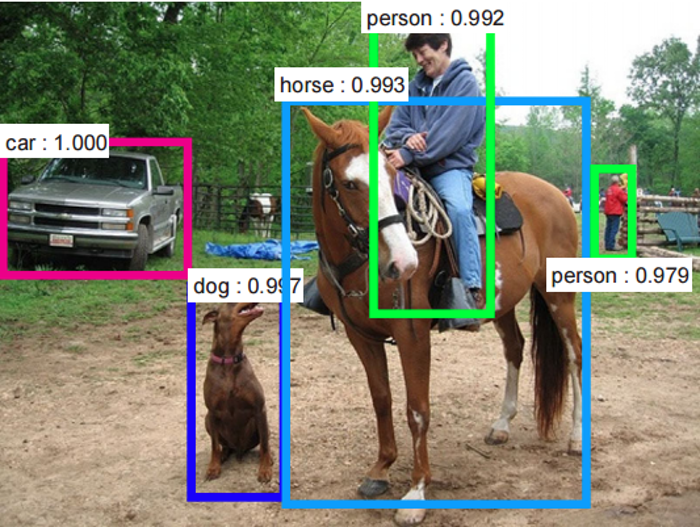
\includegraphics[scale=0.4]{images/image_classification.png}
        \caption{Image recognition by Deep Learning model \cite{faster_r_cnn}}
    \end{figure}
\end{frame}

\section{However...}

\begin{frame}[fragile]
\begin{itemize}
\item Training \alert{Deep Learning} models require a huge amount of labeled data
\vspace{0.5cm}
\item For the task of image classification on the ImageNet database, 1.2 million
    labeled images were used \cite{imagenet}
\end{itemize}
\end{frame}

%\begin{frame}[fragile]{RNN: unfold representation}
%\includegraphics[scale=0.5]{images/RNNnaive1.pdf}
%\end{frame}
%
%\begin{frame}[fragile]{RNN: cyclic representation}
%\begin{center}
%\includegraphics[scale=0.5]{images/RNNnaive2.pdf}
%\end{center}
%\end{frame}
%
%
%\section{Graph Representation}
%
%\begin{frame}[fragile]{NN as a directed graph: old version}
%\input{TikzFiles/perceptron}
%\end{frame}
%
%\begin{frame}[fragile]{Recap: sigmoid function}
%\input{TikzFiles/Sigmoid}
%\end{frame}
%
%
%\begin{frame}[fragile]{Recap: softmax function}
%\input{TikzFiles/Softmax}
%\end{frame}
%
%\begin{frame}[fragile]{NN as a directed graph: old version}
%\input{TikzFiles/OldNN1}
%\end{frame}
%
%\begin{frame}[fragile]{NN as a directed graph: old version}
%\input{TikzFiles/OldNN2}
%\end{frame}
%
%\begin{frame}[fragile]{NN as a directed graph: old version}
%\begin{center}
%\input{TikzFiles/OldNN3}
%\end{center}
%\end{frame}
%
%\begin{frame}[fragile]{Computational Graphs}
%\input{TikzFiles/Compgraph1}
%\end{frame}
%
%\begin{frame}[fragile]{Computational Graphs}
%\input{TikzFiles/Compgraph2}
%\end{frame}
%
%
%
%\begin{frame}[fragile]{Tensorflow graph}
%\begin{minted}[linenos]{python}
%import tensorflow as tf
%import numpy as np
%
%input_shape = [10,1]
%input_to_hidden_shape = [4,10]
%hidden_to_output_shape = [2,4]
%
%W1init = np.zeros(input_to_hidden_shape,
%				  dtype="float32")
%W2init = np.zeros(hidden_to_output_shape,
%				  dtype="float32")
%\end{minted}
%\end{frame}
%
%
%\begin{frame}[fragile]{Tensorflow graph}
%\begin{minted}[linenos]{python}
%graph = tf.Graph() 
%with graph.as_default():
%    x = tf.placeholder(shape=input_shape,
%                       dtype="float32") 
%    W1 = tf.get_variable(initializer=W1init)
%    v = tf.matmul(W1, x)
%    h = tf.sigmoid(v)
%    W2 = tf.get_variable(initializer=W2init)
%    z = tf.matmul(W2, h)
%    yhat = tf.nn.softmax(z)
%\end{minted}
%\end{frame}
%
%
%\begin{frame}[fragile]{Tensorboard visualization}
%\begin{center}
%\includegraphics[scale=0.255]{images/basic_tf_graph.png}
%\end{center}
%\end{frame}
%
%
%\begin{frame}[fragile]{Computational Graphs}
%\input{TikzFiles/Compgraph3}
%\end{frame}
%
%\begin{frame}[fragile]{Computational Graphs}
%\input{TikzFiles/Compgraph4}
%\end{frame}
%
%
%
%\begin{frame}[fragile]{Tensorflow graph}
%\begin{minted}[linenos]{python}
%graph = tf.Graph() 
%with graph.as_default():
%    with tf.variable_scope("x"):
%        x_prime = tf.placeholder(shape=input_shape,
%                                 dtype="float32") 
%
%    with tf.variable_scope("h"):
%        W1 = tf.get_variable(initializer=W1init)
%        v = tf.matmul(W1, x_prime)
%        h_prime = tf.sigmoid(v)
%
%    with tf.variable_scope("yhat"):
%        W2 = tf.get_variable(initializer=W2init)
%        z = tf.matmul(W2, h_prime)
%        y_prime = tf.nn.softmax(z)
%\end{minted}
%\end{frame}
%
%\begin{frame}[fragile]{Tensorboard visualization}
%\begin{center}
%\includegraphics[scale=0.27]{images/abstract_tf_graph1.png}
%\end{center}
%\end{frame}
%
%\begin{frame}[fragile]{Tensorboard visualization}
%\begin{center}
%\includegraphics[scale=0.26]{images/abstract_tf_graph2.png}
%\end{center}
%\end{frame}
%
%
%\section{RNN: the model}
%
%\begin{frame}{RNN as a graph}
%\input{TikzFiles/RNNGraphExpanded}
%\end{frame}
%
%\begin{frame}{RNN as a graph}
%\input{TikzFiles/RNNSimplified}
%\end{frame}
%
%
%\begin{frame}{Definition}
%A RNN is a function $f$ with two inputs:
%\vspace{0.2cm}
%\begin{itemize}
%\item An input vector $\vect{x}$.
%\vspace{0.1cm}
%\item A hidden vector $\vect{h}$ representing a summary of all past inputs, called \alert{state} or \alert{cell state}.
%\end{itemize}
%
%\vspace{0.2cm}
%Both inputs have a time step index $t$. The hidden unit has a recurrent definition:
%\vspace{0.2cm}
%\Large{
%\begin{equation*}
%\vect{h}^{(t)} = g(\vect{h}^{(t-1)}, \vect{x}^{(t)}; \vect{\theta})
%\end{equation*}
%}
%\end{frame}
%
%%"When the recurrent network is trained to perform a task that requires predicting the future form the past, the network typically learn to use $h^{(t)}$ as a kind of lossy summary of the task-relevant aspects of the past sequence inputs up to t"(DPB p.366)
%
%\begin{frame}{Using our example as a concrete case}
%
%\Large{
% \vspace{0.2cm}
%\begin{equation*}
%f(\vect{x}^{(t)}, \vect{h}^{(t-1)}; \vect{V}, \vect{W}, \vect{U}, \vect{c}, \vect{b}) = \vect{\hat{y}}^{(t)}
%\end{equation*}
% \vspace{0.2cm}
%\begin{equation*}
%\vect{\hat{y}}^{(t)} = softmax(\vect{V} \vect{h}^{(t)} + \vect{c})
%\end{equation*}
%\vspace{0.2cm}
% \begin{equation*}
%\vect{h}^{(t)} = g(\vect{h}^{(t-1)}, \vect{x}^{(t)}; \vect{W},\vect{U}, \vect{b})
%\end{equation*}
%\vspace{0.2cm}
%\begin{equation*}
%\vect{h}^{(t)} = \sigma(\vect{W} \vect{h}^{(t-1)} + \vect{U} \vect{x}^{(t)} + \vect{b})
%\end{equation*}
%}
%
%\end{frame}
%
%\begin{frame}{Unfolding the state equation}
%For a finite number of steps $\tau$, the recurrent definition can be unfolded. 
%For example when $\tau =3$:
%\vspace{0.2cm}
%\Large{
%\begin{align*}
%\vect{h}^{(3)}& = g(\vect{h}^{(2)}, \vect{x}^{(3)}; \vect{\theta})\\
% & = g(g(\vect{h}^{(1)}, \vect{x}^{(2)}; \vect{\theta}), \vect{x}^{(3)}; \vect{\theta})\\
% & = g(g(g(\vect{h}^{(0)}, \vect{x}^{(1)}; \vect{\theta}), \vect{x}^{(2)}; \vect{\theta}), \vect{x}^{(3)}; \vect{\theta})\\
%\end{align*}
%}
%\end{frame}
%
%\begin{frame}{Unfolding the graph}
%\input{TikzFiles/RNNSimplifiedUnfolded}
%\end{frame}
%
%\section{Language model}
%
%\begin{frame}{Definition}
%We call \alert{language model} a probability distribution over sequences of tokens in a natural language.
%
%\[
%P(x_1,x_2,x_3,x_4) = p
%\]
%
%\textbf{Used for}:
%\begin{itemize}
%\item speech recognition
%\item machine translation
%\item text auto-completion
%\item spell correction
%\item question answering
%\item summarization
%\end{itemize}
%
%
%\end{frame}
%
%\begin{frame}{How do we build these probabilities?}
%Using the chain rule of probability: 
%
%\begin{equation*}
%P(x_1,x_2,x_3,x_4) = P(x_1)P(x_2\vert x_1)P(x_3\vert x_1x_2)P(x_4\vert x_1x_2x_3)
%\end{equation*}
%
%\vspace{0.3cm}
%
%To make things simple we use a \textbf{Markovian assumption}, i.e., for a specific $n$ we assume that:
%
%\begin{equation*}
%P(x_1, \dots, x_T) = \prod_{t=1}^{T} P(x_t \vert x_1, \dots, x_{t-1}) = \prod_{t=1}^{T} P(x_{t} \vert x_{t - (n+1)}, \dots, x_{t-1})
%\end{equation*}	
%
%\end{frame}
%
%\begin{frame}{Models based on $n$-gram statistics}
%The choice of $n$ yields different models.\\
%
%\textbf{Unigram} language model ($n=1$): 
%\begin{equation*}
%P_{uni}(x_1, x_2, x_3, x_4) = P(x_1)P(x_2)P(x_3)P(x_4)
%\end{equation*}
%
%where $P(x_i) = count(x_i)$.\\
%
%\textbf{Bigram} language model ($n=2$): 
%\begin{equation*}
%P_{bi}(x_1,x_2,x_3,x_4) = P(x_1)P(x_2\vert x_1)P(x_3\vert x_2)P(x_4\vert x_3)
%\end{equation*}	
%where
%\[
%P(x_i\vert x_j) = \frac{count(x_i, x_j)}{count(x_j)}
%\]
%\end{frame}
%
%\begin{frame}{$n$-gram statistics}
%\url{https://books.google.com/ngrams}
%\vspace{0.4cm}
%
%\includegraphics[scale=0.14]{images/AI_ML.png}
%\end{frame}
%
%
%
%\begin{frame}{Evaluating a language model}
%
%\begin{itemize}
%\item \textbf{extrinsic task}: How our model perform in a NLP task such as text auto-completion.
%\begin{itemize}
%\item Time consuming.
%\end{itemize}
%\vspace{0.5cm}
%\item \textbf{intrinsic evaluation}: perplexity.
%\begin{itemize}
%\item It works only when the test data is very similar to the training data.
%\end{itemize}
%\end{itemize}
%\end{frame}
%
%\begin{frame}{Perplexity}
%\alert{Perplexity (PP)} can be thought as the weighted average branching factor of a language.\\
%
%
%Given $C= x_1, x_2, \dots, x_T$, we define the perplexity of $C$ as:
%
%\begin{align*}
%PP(C) &= P(x_1, x_2, \dots, x_T)^{-\frac{1}{T}}\\
%	  & \\
%      &= \sqrt[T]{\frac{1}{P(x_1, x_2, \dots, x_T)}}\\
%      & \\
%      &= \sqrt[T]{\prod_{i=1}^{T}\frac{1}{P(x_i \vert x_1,\dots, x_{i-1})}}
%\end{align*}
%\end{frame}
%
%\begin{frame}{Models based on $n$-gram statistics}
%\begin{itemize}
%\item Higher $n$-grams yields better performance.
%\vspace{0.7cm}
%\item Higher $n$-grams requires a lot of memory!
%\vspace{0.1cm}
%\begin{quote}
%"Using one machine \textbf{with 140 GB
%RAM for 2.8 days}, we built an unpruned
%model on 126 billion tokens."
%\end{quote}
%\begin{itemize}
%\item [] \textit{Scalable Modified Kneser-Ney Language Model Estimation} by Heafield et al.
%\end{itemize}
%\end{itemize}
%\end{frame}
%
%
%
%\begin{frame}{Languagem model as sequential data prediction}
%Instead of using one approach that is specific for the language domain, we can use a general model for sequential data prediction: a \textbf{RNN}. \\
%
%Our learning task is to estimate the probability distribution 
%
%\[
%P(x_{n} = \text{word}_{j^{*}} | x_{1}, \dots ,x_{n-1})
%\]
%
%for any $(n-1)$-sequence of words $x_{1}, \dots ,x_{n-1}$.
%\end{frame}
%
%\begin{frame}{Building the dataset}
%We start with a corpus $C$ with $T$ tokens and a vocabulary $\Vocab$.\\\
%
%Example: \textbf{Meditations in an Emergency} by Frank O'Hara.\\
%
%\begin{quote}
%\alert{Am I to become profligate as if I were a blonde? Or religious as if I were French?\\
%Each time my heart is broken it makes me feel more adventurous ... \\}
%\end{quote}
%
%\begin{itemize}
%\item $T = 645$
%\item $|\Vocab| = 347$
%\end{itemize}
%
%\end{frame}
%
%\begin{frame}{Building the dataset}
%The dataset is a collection of pairs $(\vect{x},\vect{y})$ where $\vect{x}$ is one word and $\vect{y}$ is the immediately next word. For example:
%\begin{itemize}
%\item [] $(\vect{x}^{(1)}, \vect{y}^{(1)}) =$ (Am, I).
%\item [] $(\vect{x}^{(2)}, \vect{y}^{(2)}) =$ (I, to)
%\item [] $(\vect{x}^{(3)}, \vect{y}^{(3)}) =$ (to, become)
%\item [] $(\vect{x}^{(3)}, \vect{y}^{(3)}) =$ (become, profligate)
%\item [] $(\vect{x}^{(4)}, \vect{y}^{(4)}) =$ (profligate, as)
%\item [] $(\vect{x}^{(5)}, \vect{y}^{(5)}) =$ (as, if)
%\item [] $(\vect{x}^{(6)}, \vect{y}^{(6)}) =$ (if, I)
%\item [] $\dots$
%\end{itemize}
%\end{frame}
%
%\begin{frame}{Notation}
%\begin{itemize}
%\item $\vect{E} \in \mathbb{R}^{d,|\Vocab|}$ is the matrix of word embeddings.
%\vspace{0.3cm}
%\item $\vect{x}^{(t)} \in \mathbb{R}^{|\Vocab|}$ is one-hot word vector at time step $t$.
%\vspace{0.3cm}
%\item $\vect{y}^{(t)} \in \mathbb{R}^{|\Vocab|}$ is the ground truth at time step $t$ (also an one-hot word vector).
%\end{itemize}
%\end{frame}
%
%\begin{frame}{Recap: selecting word embeddings}
%\Large{
%\begin{align*}
%  \vect{e} &= \vect{E}   \begin{bmatrix}
%                         0\\
%                         0\\
%                         \vdots \\
%                         1\\
%                         \vdots \\
%                         0
%                         \end{bmatrix}\\         
%			&= \vect{E}_{:,\;j}
%\end{align*}
% }
%\end{frame}
%
%
%\begin{frame}{The language model: graph}
%\input{TikzFiles/LanguageModelExpanded}
%\end{frame}
%
%\begin{frame}{The language model: graph}
%\input{TikzFiles/LanguageModelSimplified}
%\end{frame}
%
%
%
%\begin{frame}{The language model: equations}
%\Large{
% \vspace{0.2cm}
%\begin{equation*}
%\vect{e}^{(t)} = \vect{E}\vect{x}^{(t)}
%\end{equation*}
%\vspace{0.2cm}
% \begin{equation*}
%\vect{h}^{(t)} = \sigma(\vect{W}\vect{h}^{(t-1)}+ \vect{U}\vect{e}^{(t)}+ \vect{b})
%\end{equation*}
%\vspace{0.2cm}
%\begin{equation*}
%\vect{\hat{y}}^{(t)} = softmax(\vect{V}\vect{h}^{(t)} + \vect{c})
%\end{equation*}
%}
%\end{frame}
%
%
%\begin{frame}{The Language model: unfolding example}
%\input{TikzFiles/LanguageModelUnfolded}
%\end{frame}
%
%\begin{frame}{Recap: Entropy}
%\input{TikzFiles/Entropy1}
%\end{frame}
%
%\begin{frame}{Recap: Entropy}
%\input{TikzFiles/Entropy2}
%\end{frame}
%
%\begin{frame}{Recap: Kullback-Leibler divergence}
%\input{TikzFiles/KullbackLeibler}
%\end{frame}
%
%\begin{frame}{Recap: Cross entropy}
%\Large{
%\begin{align*}
%CE(\vect{p},\vect{q}) &= H(\vect{p}) + D_{KL}(\vect{p}||\vect{q})\\
%\vspace{0.2cm}
%&= -\sum_{i}\vect{p}_{i}\log(\vect{q}_{i})
%\end{align*}
%}
%\vspace{0.2cm}
%\begin{equation*}
%\argmin_{\vect{q}} CE(\vect{p},\vect{q}) =  \argmin_{\vect{q}} D_{KL}(\vect{p},\vect{q})
%\end{equation*}
%\end{frame}
%
%\begin{frame}{Loss function}
%At each time $t$ the point-wise loss is:
%
%\vspace{0.2cm}
%
%\begin{align*}
%L^{(t)} &= CE(\vect{y}^{(t)},\vect{\hat{y}}^{(t)})\\
%		&= - \log(\vect{\hat{y}}_{j^{*}})\\
%        &= - \log P(x^{(t+1)} = \text{word}_{j^{*}}|x^{(1)}, \dots, x^{(t)})
%\end{align*}
%
% \vspace{0.2cm}
%
%For example:
%\begin{equation*}
%L^{(3)}=- \log P(x^{(4)} = \text{become}| \text{Am}, \text{I}, \text{to})
%\end{equation*}
%\end{frame}
%
%
%\begin{frame}{Loss function}
%The loss $L$ is the mean of all the point-wise losses
%\begin{equation*}
%L=\frac{1}{T}\sum_{t=1}^{T}L^{(t)}
%\end{equation*}
%
%To give a concrete example, let's take the first sentence of the poem as $C$:
%\begin{quote}
%\alert{Am I to become profligate as if I were a blonde?}
%\end{quote}
%
%\begin{itemize}
%\item $T = 12$
%\item $|\Vocab| = 11$
%\end{itemize}
%
%\end{frame}
%
%
%\begin{frame}{Loss function: example}
%
%\begin{align*}
%        L &=-\frac{1}{12}[\log P(\text{Am} | <\text{eos}>)\\
%          &+ \log P(\text{I} | \text{Am})\\
%          &+ \log P(\text{to}| \text{Am}, \text{I})\\
%          &+ \log P(\text{become}| \text{Am}, \text{I}, \text{to})\\
%		  &+ \log P(\text{profligate}| \text{Am}, \text{I}, \text{to}, \text{become})\\
%          &+ \log P(\text{as}| \text{Am}, \text{I}, \text{to}, \text{become}, \text{profligate})\\
%          &+ \log P(\text{if}| \text{Am}, \text{I}, \text{to}, \text{become}, \text{profligate}, \text{as})\\
%          &+ \log P(\text{I}| \text{Am}, \text{I}, \text{to}, \text{become}, \text{profligate}, \text{as}, \text{if})\\
%          &+ \log P(\text{were}| \text{Am}, \text{I}, \text{to}, \text{become}, \text{profligate}, \text{as}, \text{if}, \text{I})\\
%          &+ \log P(\text{a}| \text{Am}, \text{I}, \text{to}, \text{become}, \text{profligate}, \text{as}, \text{if}, \text{I}, \text{were})\\
%          &+ \log P(\text{blonde}| \text{Am}, \text{I}, \text{to}, \text{become}, \text{profligate}, \text{as}, \text{if}, \text{I}, \text{were}, \text{a})\\
%          &+ \log P(<\text{eos}>| \text{Am}, \text{I}, \text{to}, \text{become}, \text{profligate}, \text{as}, \text{if}, \text{I}, \text{were}, \text{a}, \text{blonde})]
%\end{align*}
%
%\end{frame}
%
%\begin{frame}{Loss and Perplexity}
%Since
%\begin{align*}
%L^{(t)} & = - \log P(x^{(t+1)} |x^{(1)}, \dots, x^{(t)})\\
%& =  \log(\frac{1}{P(x^{(t+1)}|x^{(1)}, \dots, x^{(t)})})\\
%\end{align*}
%We have that:
%
%\begin{align*}
%        L &=\frac{1}{T} \sum_{t=1}^{T} L^{(t)}\\
%          &= \log\left( \sqrt[T]{\prod_{i=1}^{T}\frac{1}{P(x_i \vert x_1,\dots, x_{i-1})}} \right)\\
%          &= \log(PP(C))
%\end{align*}
%\end{frame}
%
%\begin{frame}{Loss and Perplexity}
%So another definition of perplexity is
%\vspace{0.5cm}
%\Large{
%\begin{equation*}
%2^{L} = PP(C)
%\end{equation*}
%}
%\end{frame}
%
%\section{Back Propagation}
%
%\begin{frame}{Chain rule of Calculus}
%\Large{
%\begin{itemize}
%\item $x \in \mathbb{R}$
%\item $f:\mathbb{R} \rightarrow\mathbb{R}$, $g:\mathbb{R} \rightarrow\mathbb{R}$. 
%\item $y = g(x)$
%\item $z = f(g(x)) = f(y)$
%\end{itemize}
%
%\[
%\frac{dz}{dx} = \frac{dz}{dy} \frac{dy}{dx} 
%\]
%}
%\end{frame}
%
%\begin{frame}{Chain rule: example}
%\Large{
%\begin{itemize}
%\item $y = x^2$
%
%\vspace{0.3cm}
%
%\item $z = \log(y)$
%\end{itemize}
%
%\vspace{0.5cm}
%
%\[
%\frac{dz}{dx} = \frac{dz}{dy} \frac{dy}{dx} = \frac{1}{x^2}2x = \frac{2}{x}
%\]
%}
%\end{frame}
%
%\begin{frame}{Chain rule: graph}
%\input{TikzFiles/BackPropScalar}
%\end{frame}
%
%\begin{frame}{Chain rule: vector notation}
%\Large{
%\begin{itemize}
%\item $\vect{x} \in \mathbb{R}^{m}$
%\item $\vect{y} \in \mathbb{R}^{n}$
%\item $f:\mathbb{R}^{n} \rightarrow\mathbb{R}$, $g:\mathbb{R}^{m} \rightarrow\mathbb{R}^{n}$. 
%\item $\vect{y} = g(\vect{x})$
%\item $\vect{z} = f(g(\vect{x})) = f(\vect{y})$
%\end{itemize}
%\[
%\frac{\partial z}{\partial x_{i}} =\sum_{j} \frac{\partial z}{\partial y_{j}} \frac{\partial y_{j}}{\partial x_{i}} 
%\]
%}
%\end{frame}
%
%\begin{frame}{Chain rule: vector notation}
%
%\Large{
%\begin{itemize}
%\item $\vect{x} \in \mathbb{R}^{m}$
%\item $\vect{y} \in \mathbb{R}^{n}$
%\item $f:\mathbb{R}^{n} \rightarrow\mathbb{R}$, $g:\mathbb{R}^{m} \rightarrow\mathbb{R}^{n}$. 
%\item $\vect{y} = g(\vect{x})$
%\item $\vect{z} = f(g(\vect{x})) = f(\vect{y})$
%\end{itemize}
%\[
%\grad{\vect{x}}{z} = \left(\frac{\partial \vect{y}}{\partial \vect{x}}\right)^{T}\grad{\vect{y}}{z}
%\]
%}
%\end{frame}
%
%\begin{frame}{Recap: gradient}
%\Large{
%\begin{align*}
%  \grad{\vect{y}}{z} &= \begin{bmatrix}
%                         \frac{\partial z}{\partial y_{1}} \\
%                         \frac{\partial z}{\partial y_{2}} \\
%                         \vdots \\
%                         \frac{\partial z}{\partial y_{n}}
%                         \end{bmatrix}
%\end{align*}
% }
%\end{frame}
%
%\begin{frame}{Recap: Jacobian matrix}
%\Large{
%\[
%\frac{\partial \vect{y}}{\partial \vect{x}} =
%\begin{bmatrix} 
%
%\frac{\partial y_{1}}{\partial x_{1}} & \frac{\partial y_{1}}{\partial x_{2}} & \dots & \frac{\partial y_{1}}{\partial x_{m}} \\
%
%\vdots & \ddots &\dots & \vdots \\
%
%\frac{\partial y_{n}}{\partial x_{1}} &\frac{\partial y_{n}}{\partial x_{2}} & \dots&\frac{\partial y_{n}}{\partial x_{m}} 
%
%\end{bmatrix}
%\]
% }
%\end{frame}
%
%\begin{frame}{Chain rule: example}
%\Large{
%\begin{itemize}
%\item $\vect{y} = \vect{W}\vect{x}$
%
%\vspace{0.3cm}
%
%\item $z = \vect{b}^{T}\vect{y}$
%\end{itemize}
%
%\vspace{0.5cm}
%
%\[
%\grad{\vect{x}}{z} =  \vect{W}^{T}\vect{b}
%\]
%}
%\end{frame}
%
%
%\begin{frame}{Chain rule: graph}
%\input{TikzFiles/BackPropVector}
%\end{frame}
%
%\begin{frame}{Computing the gradient in a RNN}
%\begin{itemize}
%\item We simple apply the back-propagation algorithm to the unrolled computational graph.
%
%\vspace{0.5cm}
%
%\item Since each subgraph represents a time step, the application of back-propagation in this model is also called \alert{Back-Propagation Through Time}.
%\end{itemize}
%\end{frame}
%
%
%\begin{frame}{A very simple RNN}
%
%\Large{
%\begin{equation*}
%\vect{a}^{(t)} = \vect{W} \vect{h}^{(t-1)} + \vect{U} \vect{x}^{(t)}
%\end{equation*}
%
%\vspace{0.1cm}
%
%\begin{equation*}
%\vect{h}^{(t)} = \sigma(\vect{a}^{(t)})
%\end{equation*}
%
%\vspace{0.1cm}
%
%\begin{equation*}
%\vect{o}^{(t)} = \vect{V} \vect{h}^{(t)}
%\end{equation*}
%
%\vspace{0.1cm}
%
%\begin{equation*}
%\vect{\hat{y}}^{(t)} = softmax(\vect{o}^{(t)})
%\end{equation*}
%}
%
%\end{frame}
%
%
%\begin{frame}{RNN time unfolding}
%\input{TikzFiles/rnn-time-unfolding}
%\end{frame}
%
%\begin{frame}{Recap: Hadamard product}
%\Large{
%\begin{equation*}
%(\vect{x} \circ \vect{y})_{i} = \vect{x}_{i} \vect{y}_{i} 
%\end{equation*}
%
%\vspace{0.5cm}
%
%\begin{equation*}
%(\vect{x} \circ \vect{y}) = diag(\vect{y})\vect{x} 
%\end{equation*}
% }
%\end{frame}
%
%\begin{frame}{Chain rule: RNN graph}
%\input{TikzFiles/rnn-backprop}
%\end{frame}
%
%
%\begin{frame}{Back Propagation Throught Time}
%\input{TikzFiles/rnn-backprop-through-time}
%\end{frame}
%
%\begin{frame}{Back Propagation Through Time}
%The gradients on $\vect{V}$, $\vect{W}$ and $\vect{U}$ are:
%\vspace{0.3cm}
%\Large{
%\begin{equation*}
%\grad{\vect{V}}{L^{(\tau)}} = \outerp{\grad{\vect{o}^{(\tau)}}{L^{(\tau)}}}{\vect{h}^{(\tau)}} 
%\end{equation*}
%
%
%\begin{equation*}
%\grad{\vect{W}}{L^{(\tau)}} = \sum_{t=1}^{\tau}\grad{\vect{W}^{(t)}}{L^{(\tau)}}
%\end{equation*}
%
%\begin{equation*}
%\grad{\vect{U}}{L^{(\tau)}} = \sum_{t=1}^{\tau}\grad{\vect{U}^{(t)}}{L^{(\tau)}}
%\end{equation*}
%}
%\end{frame}
%
%\section{Vanishing or Exploding Gradient}
%\input{equations}
%
%\begin{frame}{Taking a closer look}
%With some notation we can simplify these gradients as follows:
%\begin{eqnarray*}
%\grad{\vect{U}^{(3)}}{L^{(3)}} = \vect{c}{\vect{x}^{(3)}}^{T}
%\end{eqnarray*}
%
%\begin{eqnarray*}
%\grad{\vect{U}^{(2)}}{L^{(3)}} = \outerp{diag(\vect{b}^{(2)}) \vect{W}^{T} \vect{c}}{\vect{x}^{(2)}}
%\end{eqnarray*}
%
%\begin{eqnarray*}
%\grad{\vect{U}^{(1)}}{L^{(3)}} = \outerp{\left(diag(\vect{b}^{(1)}) \vect{W}^{T} \right) \left(diag(\vect{b}^{(2)}) \vect{W}^{T}\right) \vect{c}}{\vect{x}^{(1)}}
%\end{eqnarray*}
%\end{frame}
%
%\begin{frame}{Taking a closer look}
%
%
%\[
%\grad{\vect{U}^{(1)}}{L^{(\tau)}}
%\]
%\[
%=
%\]
%\[
%\outerp{\left(diag(\vect{b}^{(1)}) \vect{W}^{T} \right) \left(diag(\vect{b}^{(2)}) \vect{W}^{T}\right) \dots \left(diag(\vect{b}^{(\tau-1)}) \vect{W}^{T}\right)\vect{c}}{\vect{x}^{(1)}}
%\]
%
%\vspace{0.5cm}
%
%\textbf{Gradient for further time steps will have more matrix products using $diag(\vect{b}) \vect{W}^{T}$.
%}\end{frame}
%
%\begin{frame}{Vanishing}
%
%If we initialize $\vect{W}$ such that $||\vect{W}|| < 1$, the gradient for further time steps will be very small (\alert{vanishing problem}).
%
%\vspace{0.8cm}
% \url{https://www.youtube.com/watch?v=xAl8fu8myW0}
%
%
%\end{frame}
%
%
%
%\begin{frame}{Exploding}
%
%If $||\vect{W}|| > 1$, the gradient for further time steps will be larger and larger (\alert{exploding problem}).
%
%\vspace{0.8cm}
% \url{https://www.youtube.com/watch?v=dqW-jw5qKK8}
%
%
%\end{frame}
%
%
%\begin{frame}{The vanishing problem}
%
%The gradients from the steps closed to $\tau$ (the last step) have more influence than the ones very far back.\\
%
%This is bad for capturing \alert{long-term dependecies}.
%\end{frame}
%
%\begin{frame}{Possible solutions (hacks)}
%\begin{itemize}
%\item Clip gradients to a maximum value.
%\vspace{0.4cm}
%\item Choosing the right activation functions, e.g. ReLU.
%\vspace{0.4cm}
%\item Initialize weights to the identity matrix.
%\vspace{0.4cm}
%\item LSTM (Long Short-Term Memory), GRU (Gated Recurrent Unit), etc
%\end{itemize}
%\end{frame}
%
%
%\section{Implementation}
%
%\begin{frame}{Truncated Back Propagation}
%\url{www.tensorflow.org/versions/master/tutorials/recurrent}
%\begin{quote}
%"By design, the output of a recurrent neural network (RNN) depends on arbitrarily distant inputs. Unfortunately, this makes backpropagation computation difficult. In order to make the learning process tractable, \alert{it is common practice to create an 'unrolled' version of the network, which contains a fixed number (num\_steps) of LSTM inputs and outputs}."
%\end{quote}
%\end{frame}
%
%\begin{frame}[fragile]{Tensorflow implementation}
%\begin{minted}[linenos]{python}
%self.rnn_outputs = []
%
%initialshape = (self.batch_size, self.hidden_size)
%Wshape = (self.hidden_size, self.hidden_size)
%Ushape = (self.embed_size, self.hidden_size)
%Vshape = (self.config.hidden_size, self.vocab_size)
%
%with tf.variable_scope("memory"):
%    self.initial_state = tf.zeros(initialshape)
%
%with tf.variable_scope("hidden"):
%    self.W = tf.get_variable("W", shape=Wshape)
%    self.input_weights = init_wb(Ushape, "input_weights")
%\end{minted}
%\end{frame}
%
%\begin{frame}[fragile]{Tensorflow implementation}
%\begin{minted}[linenos]{python}
%previous_h = self.initial_state
%for i, tensor in enumerate(self.inputs):
%          # len(self.inputs) = num_steps
%    with tf.variable_scope("RNN", reuse=True):
%        drop_tensor = tf.nn.dropout(tensor,
%                                    self.dropout_placeholder)
%        h = (tf.matmul(previous_h, self.W) +
%             affine_transformation(drop_tensor,
%                                   self.input_weights))
%        h = tf.nn.dropout(tf.sigmoid(h),
%                          self.dropout_placeholder)
%        self.rnn_outputs.append(h)
%        previous_h = h
%        if i == (len(self.inputs) - 1):
%            self.final_state = h
%\end{minted}
%\end{frame}
%
%\begin{frame}[fragile]{Tensorflow implementation}
%\begin{minted}[linenos]{python}
%with tf.variable_scope("Projection_layer"):
%    self.output_weights = init_wb(Vshape, "output_weights")
%    self.logits = [affine_transformation(tensor,
%                                         self.output_weights)
%                   for tensor in self.rnn_outputs]
%\end{minted}
%\end{frame}
%
%\begin{frame}{MytwitterBot: TrumpBot}
%\url{https://github.com/felipessalvatore/MyTwitterBot}
%\begin{center}
%\includegraphics[scale=0.24]{images/TrumpBot.png}
%\end{center}
%\end{frame}
%
%\begin{frame}{MytwitterBot: SakaBot}
%\url{https://github.com/felipessalvatore/MyTwitterBot}
%\begin{center}
%\includegraphics[scale=0.24]{images/SakaBot.png}
%\end{center}
%\end{frame}
%
%
%
%\section{Conclusion}
%
%\begin{frame}{What's next?}
%After some experiments with the hyper parameters my best result on the \alert{Penn Treebank (PTB)} corpus was
%
%\vspace{0.5cm}
%
%\begin{figure}
%\begin{center}
%\begin{tabular}{|c|c|c|}
%\hline
%\cellcolor{blue!60}Model & \cellcolor{blue!60}Val & \cellcolor{blue!60}Test  \\ \hline
%Mikolov et al (2011)\cite{Mikolov11} & $163.2$  & $149.9$ \\ \hline
%\end{tabular}
%\end{center}
%\end{figure}
%\end{frame}
%
%\begin{frame}{LSTM}
%\url{http://blog.ycombinator.com/jeff-deans-lecture-for-yc-ai/}
%
%\begin{center}
%\includegraphics[scale=0.45]{images/JeffDeanLectureforYCAI.pdf}
%\end{center}
%\nocite{DeepLearningbook}
%
%\end{frame}
%
%
%\begin{frame}{LSTM: \url{https://arxiv.org/abs/1708.02182}}
%
%\begin{center}
%\includegraphics[scale=0.34]{images/SocherPTB.png}
%\end{center}
%
%\end{frame}
%
%
\begin{frame}[allowframebreaks]{References}

  \bibliography{demo}
  \bibliographystyle{abbrv}

\end{frame}

\end{document}
